\documentclass{l4proj}

%Packages
\usepackage{natbib}

\begin{document}
\title{Augmented Reality Android Gym App}
\author{David Benicek 2073063b}
\date{\today}
\maketitle

\begin{abstract}
Something will go here.
\end{abstract}

\educationalconsent
%
%NOTE: if you include the educationalconsent (above) and your project is graded an A then
%      it may be entered in the CS Hall of Fame
%
\tableofcontents
%==============================================================================

\chapter{Introduction}
\pagenumbering{arabic}
\section{Motivation}
Frequent exercise and a healthy lifestyle have recently become an integral part of the western culture. Indeed, last year in America more people have exercised on a regular basis then ever before \cite{USexercise}. As people begin to adopt this new and healthy lifestyle, it is immediately obvious that there are two distinct periods during which there seems to be a lack of coherent information. These are at the very beginning when a person begins to exercise for the first time and when a person begins to plateau and starts to experience diminishing returns for their workouts due to a lack of variation in their routine. It is important to note that a lack of coherent information does not necessarily mean a lack of data but instead a lack of a singular consensus in the midst of conflicting information, fad diets, ill-informed advice and 'bro science'. Therefore, it seems that there is a need for a singular portal to which both beginners and experienced gym goers alike can refer to for information regarding exercise.  

\section{Aim} \label{sec:aim}
Tackling the entire topic of fitness in one application would be extremely difficult, if not impossible. Due to this we are going to narrow down the focus and seek to add value to users while they are in the gym. The aim of the application will be to help users understand how to use gym equipment, suggest a range of exercises that can be carried out on a given piece of equipment and demonstrate how to perform the exercise with correct and safe form. 

One of the main goals of the app is for it to be responsive to the user's environment and heavily interactive so that the user has an immersive experience. An immersive experience will keep users engaged with the app however there is a balance to be drawn here. Since the gym is a potentially dangerous environment, the design of the app must make sure that users do not loose track of their surroundings completely. One possible way of striking this balance is through augmented reality (AR). AR would allow us to give a somewhat immersive experience by super imposing realistic human models on the device's screen without the need for a completely virtualized reality. Similar applications of AR have been trialed in education, construction, sports and medicine to various degrees of success. A review of literature regarding previous work done with AR can be found in section \ref{sec:litrew}.

\section{Outline}
In this document we are going to explore the different steps taken in the development of the augmented reality gym app. First, we will review relevant literature in order to be able to make informed decisions concerning requirements and constraints. Requirements elicited from discussions with the Glasgow University Sports Association (GUSA) will also be review and summarized. Following, will be a discussion of the possible designs of the app from both a user experience and user interface aspect. Later we will go trough the steps in implementation and testing, outlining the procedure and any major problems along the way. Finally, we will draw the document to a close with a conclusion, followed by an evaluation, where we will address to what extend the main objectives of the project were achieved and reflect on what could have been done differently for future reference. 

\chapter{Requirements}


\section{Review of previous work} \label{sec:litrew}
The term 'augmented reality' was coined by Tom Caudell, a Boeing researcher in 1990 \cite{rauterberg_history_2002}. Caudell first envisioned augmented reality as transparent screens that would be used to simply display complicated drawings and plans. AR has evolved tremendously since the 1990s and with it so has it's definition. In order to understand augmented reality we first have to address the concept of mixed reality. Mixed reality is the overarching concept of blending the real and virtual worlds \cite{milgram_taxonomy_1994}. Within the field of mixed reality there are many branches which lie on a spectrum between a non-manipulated, real environment and a fully digital environment created in virtual reality. The spectrum can be see in figure \ref{fig:ar-spectrum} and it is important to note that immersion increases as we move to the right from the real environment to the virtual environment. Augmented reality sits in the left center of the spectrum and can be broadly defined as technologies that project digital materials onto real world objects"\cite{cuendet_designing_2013}. Importantly, augmented reality integrates  "3D virtual objects ... into a 3D real environment in real time"\cite{azuma_survey_1997}. The added virtual content is obviously superimposed and the distinction between real and virtual is clear, unlike with other technologies further down the spectrum. For example, on the extreme right of the spectrum is virtual reality, which fully replaces the real world with computer generated scenes and aims to mimic the real world \cite{tamura_mixed_2001}. This research is going to focus only on augmented reality since it provides just enough immersion to exploit phenomenon such as situativity (which will be explained later) and yet does not cause the user to be completely absorbed into the application nor does it require additional equipment. 

\begin{figure}
\centering
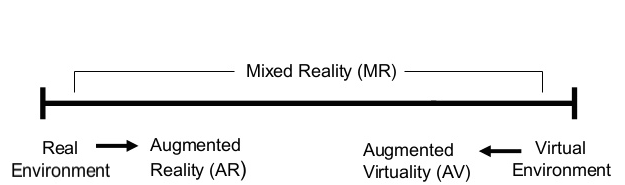
\includegraphics[scale=1]{images/ar-spectrum.png}
\caption{A spectrum overview of mixed reality technologies (Milgran 1994)}
\label{fig:ar-spectrum}
\end{figure}

AR has been used in a number of disciplines, ranging from medicine to entertainment to construction.\cite{azuma_recent_2001} (TODO: page 3-9). It seems that there has been no previous research done on the possible application of AR in the fitness sector and therefore we will draw on insights from other applications of AR. We will especially focus on pedagogical applications of AR with the hope of drawing parallels between teaching a class and instructing users to perform exercises in the gym. 

Eventhough AR in classrooms has been previously used on desktop machines \cite{iordache_comparison_2009}, it's true power has only been unleashed recently, as the shrinking of technologies has allowed AR to migrate from desktop to mobile devices \cite{squire_augmented_2007}. Squire and Klopfer studied four different groups of students using an AR game in which students took on the role of environmental detectives. One of the main advantages of AR that were highlighted in their research was the ability to trigger the recollection of preexisting knowledge \cite{squire_augmented_2007}. "Learning is contextual" \cite{liestol_learning_2011} and so, by placing students in a familiar environment, they are likely to recollect what they previously learnt in that same location. This is supported by the pedagogical psychologist Greeno who put forward the theory of situativity, which argues that immersing oneself in the context of a situation aids with its understanding and recolection of previous relevant information\cite{greeno_situativity_1998}. Dede has studied full virtual reality and has noted the possitive effects of immersion on the transfer of knowledge from theory into practice in the real world\cite{dede_immersive_2009}. Importantly, according to Dede "lesser degrees of immersion can still provide situated learning" and all the benefits that come with it\cite{dede_immersive_2009}. Situativity will be fully exploited in our gym application. By simply by placing users in the correct environment, they will have a higher chance of recalling and learning the correct form of an exercise. All in all, the advantage of situativity as well as the evidence that suggests AR is an effective way to visualise information and instructions \cite{squire_augmented_2007} suggest it is a suitable technology for teaching and for our gym application.

Radu expanded on the initial research of using of AR in classrooms. Similary to Squire and Klopfer, Radu noticed a number of specific positive impacts that AR can have on learning \cite{radu_why_2012}. In Radu's experiment, AR increased understanding and the long-term retention of taught content as well as the student's motivation\cite{radu_why_2012}. Unfortunately, Radu also noticed some usability difficulties and fluctuating levels of understanding between students \cite{radu_why_2012}, hinting at the fact that design and usability are key in AR applications. Others, such as Liestøl have realized the possible difficulties of adoption AR in the classroom but has stated that "the threshold for entering this technology is not insurmountable - it is actually relatively easy". Indeed, the benefits that AR brings, such as improved learning, retention and motivation are impressive but they do come at a cost. The initial adoption of AR may bring with it some issues but if resolved, the prospects of AR truly impressive. In  pedagogy, most teachers would need to create their own AR application, or use one that is specifically targeted at their syllabus and at what they are trying to teach students, however, in the context of the gym app, there is no need for each individual user to re-create the app since the exercises they are trying to learn are uniform. This removes a significant barrier to the use of AR in the gym context and all that is left to do is for the user to familiarize themselves with the AR app - just as they would with any other non-AR application. 

Mobile AR applications allow the users to move around the scene and explore different angles and perspectives of the rendered object, catering to a more dynamic and interactive learning experience\cite{fitzgerald_augmented_2013}\cite{dede_immersive_2009}. Kerawalla et al. carried out an experiment where AR was assessed against other, more traditional, methods to teach a class about the solar system\cite{kerawalla_making_2006}. In total, 133 children grouped in different classes attended the experiment. Each class was split into three groups and each group was then ran through two sessions of teaching, using different teaching methods. There were four variations to the teaching styles: Using AR by a teacher who is an expert in AR, using AR by the classes own teacher who had no prior experience with AR, using a lecture and book combination and finally using the BBC ReviseWise website where kids work independently at the computer. The debate during class was analysed and the teachers interviewed a few days after the class occurred. One of the main outcomes of the experiment was that teachers saw the value in AR making "traditionally inaccessible subject matter available to the children"\cite{kerawalla_making_2006} and thus enriching their learning experience. Kerawalla et al. did not go as far as to assess the amount kids learned during the AR session in comparison to the sessions taught in a traditionally style but one teacher highlighted that using AR, a student "can see that picture in his head rather than just being told it, or like with a globe and a torch and having to work out what stands for what"\cite{kerawalla_making_2006}. All in all, the teachers found that AR made "the  subject  matter  accessible  and real" which will is the goal of the gym application and therefore AR seems to be a good choice. 

One of the main issues with AR is allignment \cite{sood_pro_2012}. Object recognition, especially on mobile devices, does not yet have the needed fidelity to be able to distinguish the same object in different variations. For example, object recognition could be used to recognize a bench in the gym however, it will only ever be able to recognize that specific type of bench. In a different gym, with different benches or even with the same bench but different lighting, shadows and perhaps colour, object recognition will do us no good. One possible solution, proposed by Rekimoto and Ayatsuka is to have visual tags on the objects and use these to identify them \cite{rekimoto_cybercode:_2000}. We can group objects that fall in the same category by giving them the save tag and placing it in the correct area. We then use image recognition to recognize the tag and use it as an anchor for our augmented reality overlay. By tracking the position and size of the visual tag we can move and size our augmentation accordingly.  

Balog et al. took a different approach to AR and decided to use AR glasses and a 'paddle' to point at and select virtual objects as a part of a class room exercise. There were several issues identified in their research, most important were the inability to select every element due to overlapping and low fidelity, the paddle blocking the view of the user and a lack of feedback\cite{balog_augmented_2007}. Despite some of the shortcomings, a group of 32 students scored the AR exercise as exiting (4.16 on a 5 point scale) and gave scores of 4.38, 4.31 and 4.34 respectively for understanding the lesson, easy operation and readability of presented information\textbf{•}. On the other hand, interacting with the virtual objects using the 'paddle' was ranked lower, at only 3.06\cite{balog_augmented_2007}, Looser et al. also experimented with different input methods, testing selection with a virtual hand and with two methods of using virtual pointers\cite{looser_evaluation_2007}. Both uses of pointers performed poorly, with error rates deviating around 45\%\cite{looser_evaluation_2007}. The virtual hand performed much better but still suffered from a 20\% miss rate\cite{looser_evaluation_2007}, which suggests it is better to choose  more traditional methods of user interaction instead of opting for a virtual interface. Based on this, the gym application will implement a touch screen interface with standard onscreen buttons rather than using a fully augmented virtual interface. 

Perhaps the most important issue when creating a phone app in general and an AR app in particular is the issue of attention tunneling \cite{radu_why_2012} \cite{biocca_attention_2007}. Attention tunnels, such as oncreen indicator that point the user in the correct direction have previously been used with impressive sucess\cite{biocca_attention_2007}. In one experiment, attention funnels increased "the consistency of the user’s search by 65\%,  increased search speed by 22\%, and decreased mental workload by 18\%" \cite{biocca_attention_2007}. Clearly attention funnels can extremely useful but since using AR is a relatively immersive experience and we must take care to draw the users attention to the appropriate stimulai and objects in order for them to not completely loose track of their environment - especially in the gym. Biocca et al. have pointed out issues with attention funneling in mobile interfaces in general, stating that "the attention demands of current interfaces such as cellular phones and PDAs may play a significant role in automobile accidents". Some AR applications such as Pokemon Go have solved the issue of attention tunneling through pop ups that remind the user to stay aware of their surroundings \cite{hollister_drivers_2016}. A similar approach should be adopted in our application to ensure the users safety and must be one of the high priority requirements.

On the topic of safety, the demonstrated exercises could pose a health and safety risk to the users. There are often many different ways to carry out a single exercise and frequently there is no consensus on the best approach. Most of the times there will be an ideal motor pattern to lift the most weight efficiently, in theory, however when a user tries to recreate this, they might be put in a compromising position. Take, for example, the deadlift (picking up a bar from the floor and finishing in a standing position with the bar mid thigh). Within the app, we may demonstrate that the safest starting position is from a half-squat where the thighs make a 25° angle with the floor. This may indeed be the safest position for someone with a perfectly proportionate body, but if somebody has shorter arms and longer legs, they may need to squad down further to reach the bar and be in a strong position. If such a user were to follow our instructions too closely they may round their back too much in order to reach down to the bar and end up hurting themselves. If a user was so inclined, they could blame the app for providing unsafe instructions to them. One possible solution to this problem is to have a disclaimer either as a pop up within the app or on the loading screen. If a user is clearly made aware that the demonstrated form for each exercise is only approximate and shows what the creators deemed most efficient, then there should be no liability issues. 

\subsection{Meeting with GUSA}
When developing an app of any kind it is important to consider how you are going to market and distribute the finished product. This question is particularly interesting in our context because the app needs some real-life components (markers) to work and therefore needs to be pitched to both daily users and gym owners. One of the first steps that I carried out, before doing much research into technologies and development was to arrange a meeting with the Glasgow University Sports Association (GUSA). I pitched my idea to the president of GUSA in an email and was able to arrange a meeting both with GUSA president and the Sport Development Manager at Glasgow University. The meeting 	was held on the 26th of July 2016 and yielded a number of interesting requirements and points of discussion, many of which I had not previously considered. 

One point of discussion was the issue of liability. The main goal of the app is to demonstrate what perfect form of an exercise looks like, however there are conflicting views as to what 'perfect' form for an exercise is. One expert might argue one way and another might be completely opposed which will mean that the app will have to choose a side. If the chosen side is eventually found to be incorrect, or worse, dangerous there could be options of liability. A potential solution would be to show a disclaimer on or during app launch that notifies the user that all demonstrations of form are approximate and that the user should contact an expert if they are unsure how to properly and safely perform an exercise. 

GUSA was cautious about how the app is going to be distributed and marketed since they are themselves working on a designated GUSA app and are also pushing the LifeFitness app to their customers. The main concern was that by having too many apps marketed in the gym, customers would be overwhelmed and end up using none of the apps. It was decided that in order to solve this dilemma, my app would not be distributed by GUSA nor will it have any relation to GUSA. Instead the Glasgow University gym will simply be an environment for testing. 


\chapter{Design}
\section{User Experience}
The quick brown fox jumped over the lazy dog.
The quick brown fox jumped over the lazy dog.
The quick brown fox jumped over the lazy dog.
The quick brown fox jumped over the lazy dog.
\section{User Interface}
The quick brown fox jumped over the lazy dog.
The quick brown fox jumped over the lazy dog.
The quick brown fox jumped over the lazy dog.
The quick brown fox jumped over the lazy dog.

\chapter{Implementation}
The development of an augment reality phone application sounds quite daunting at first. The image recognition, 3D object imaging and use of sensors and mathematical calculations to pivot the projected image are undoubtedly complex however, there are many libraries and tools that allow us for the abstraction of the complex and intricate work and allow us to focus on the core app development. Despite this, the initial learning curve to find, set up and get started with all the tools and technologies is quite steep. In this section we are first going to explore the numerous tools used throughout the project, justify their selection and talk about how they are used. Later we will talk about some of the challenges that had to be overcome during the implementation process. 
\subsection{Technologies used}
\subsubsection{Git}
One of the first tools that was set up as a part of the project was the Git version control system. Git is usually used in the open source community or within teams to allow easy integration between contributors. In our case Git is used to keep a backup of old versions of the project and to share the progress of the project with the project supervisor. There are many other version control systems such as SVN or Merculiar. Git was chosen due to my familiarity with it and due to the fact that in most cases it is an industry standard.
	
\subsubsection{Vuforia}
Vuforia is one of the many open source augmented reality libraries \cite{vuforia}. Vuforia provides an online interface where you can upload different images which are then analysed for specific feature patterns that are used for matching. For example figure \ref{fig:coca_cola_features} show the feature patterns of a CocaCola logo. A collection of such targets can be exported as a database and later used in Unity for matching using optical recognition \cite{vuforia_unity}.
\begin{figure}
\centering

\includegraphics[scale=1]{images/coca_cola_features.png}
\caption{Patterns of features on the CocaCola logo.}
\label{fig:coca_cola_features}
\end{figure}

Vuforia allows us to create markers but it is also a plugin for Unity and an SDK that is used in native Android code development \cite{vuforia_unity}.

\subsubsection{Unity}


\subsubsection{MakeHuman}


\subsection{Trials and Tribulations }
 
\chapter{Testing}

\chapter{Conclusion}

\chapter{Evaluation}

%\vspace{-7mm}
\begin{figure}
\centering
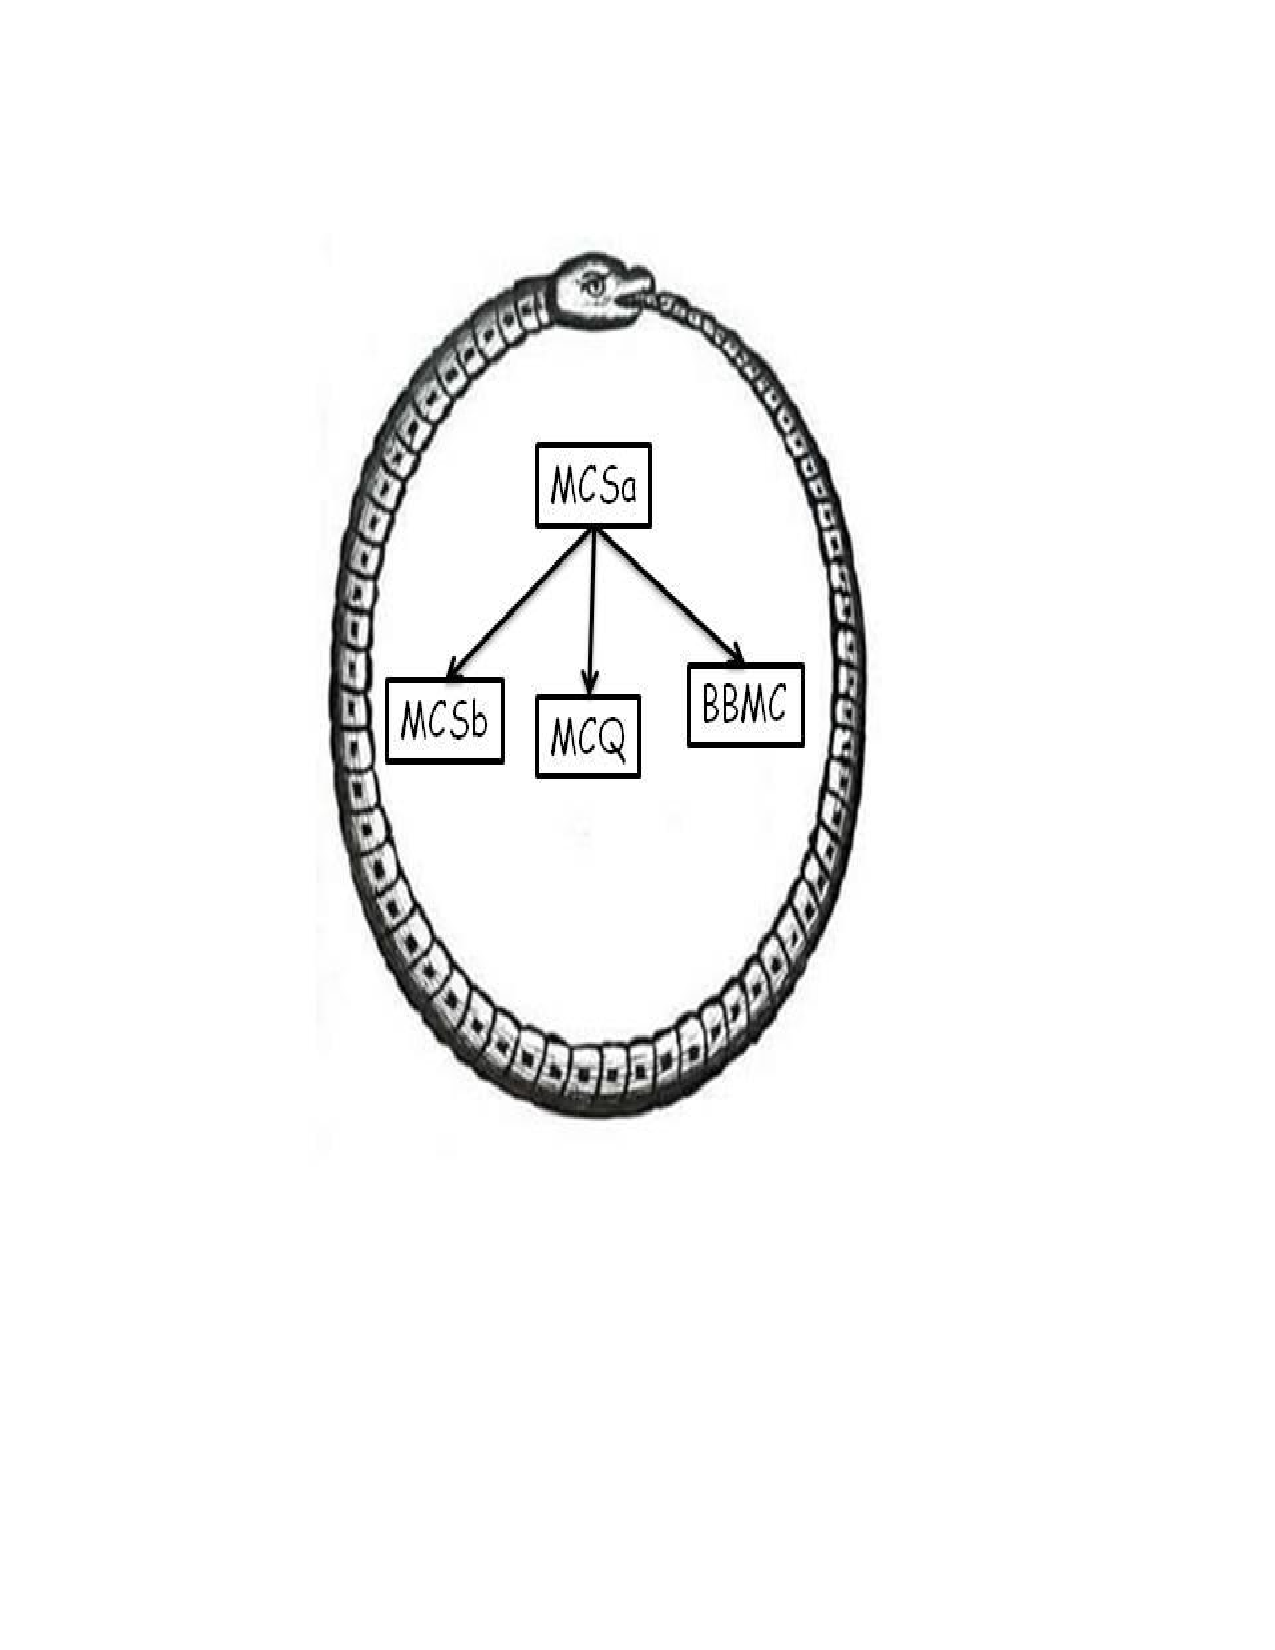
\includegraphics[height=9.2cm,width=13.2cm]{uroboros.pdf}
\vspace{-30mm}
\caption{An alternative hierarchy of the algorithms.}
\label{uroborus}
\end{figure}



%%%%%%%%%%%%%%%%
%              %
%  APPENDICES  %
%              %
%%%%%%%%%%%%%%%%
\begin{appendices}

\chapter{Running the Programs}
An example of running from the command line is as follows:
\begin{verbatim}
      > java MaxClique BBMC1 brock200_1.clq 14400
\end{verbatim}
This will apply $BBMC$ with $style = 1$ to the first brock200 DIMACS instance allowing 14400 seconds of cpu time.

\chapter{Generating Random Graphs}
\label{sec:randomGraph}
We generate Erd\'{o}s-R\"{e}nyi random graphs $G(n,p)$ where $n$ is the number of vertices and
each edge is included in the graph with probability $p$ independent from every other edge. It produces
a random graph in DIMACS format with vertices numbered 1 to $n$ inclusive. It can be run from the command line as follows to produce 
a clq file
\begin{verbatim}
      > java RandomGraph 100 0.9 > 100-90-00.clq
\end{verbatim}
\end{appendices}

%%%%%%%%%%%%%%%%%%%%
%   BIBLIOGRAPHY   %
%%%%%%%%%%%%%%%%%%%%

\bibliographystyle{plain}
\bibliography{bib}

\end{document}
